Os experimentos realizados permitiram comparar o desempenho de diferentes algoritmos de regressão e classificação multiclasse em cenários distintos, utilizando métricas médias ao longo de múltiplas execuções. A seguir, os principais resultados comparativos para cada base de dados e cenário são discutidos, com referência direta a cada figura para facilitar a análise visual.

\subsection{Análise dos Resultados de Regressão}

No conjunto Energy Efficiency, observa-se que alguns modelos apresentam menor erro médio (RMSE e MAE), enquanto outros se destacam pelo maior poder explicativo ($R^2$). As Figuras~\ref{fig:energy_rmse}, \ref{fig:energy_mae} e \ref{fig:energy_r2} ilustram essas diferenças, permitindo identificar visualmente qual modelo apresenta menor erro e qual possui maior capacidade explicativa, auxiliando na escolha do algoritmo mais adequado conforme a métrica de interesse.

\begin{figure}[H]
    \centering
    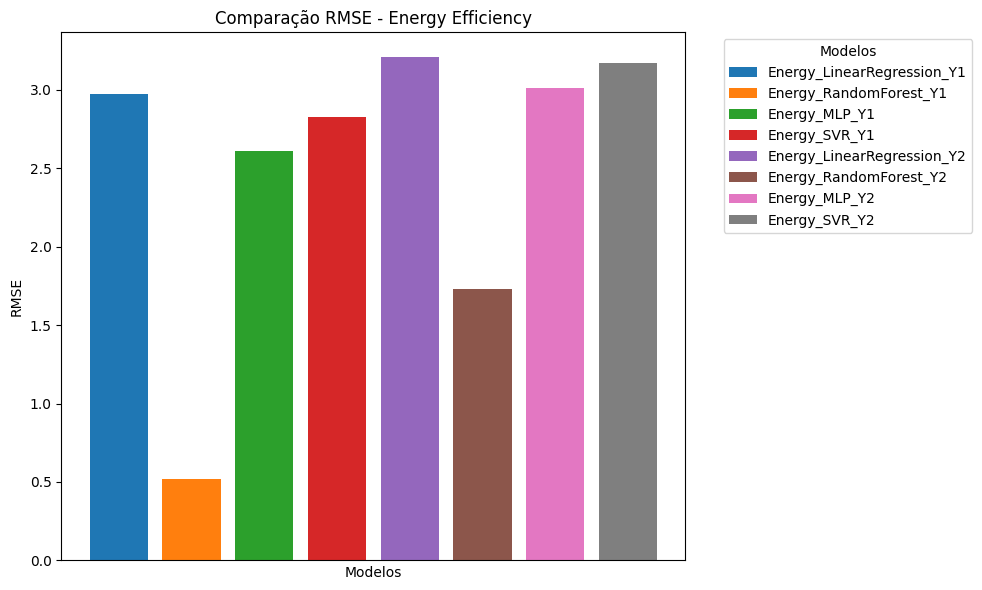
\includegraphics[width=0.45\textwidth]{../graficos/comparacao_rmse_energy.png}
    \caption{Boxplot do RMSE médio entre algoritmos de regressão para Energy Efficiency.}
    \label{fig:energy_rmse}
\end{figure}

\begin{figure}[H]
    \centering
    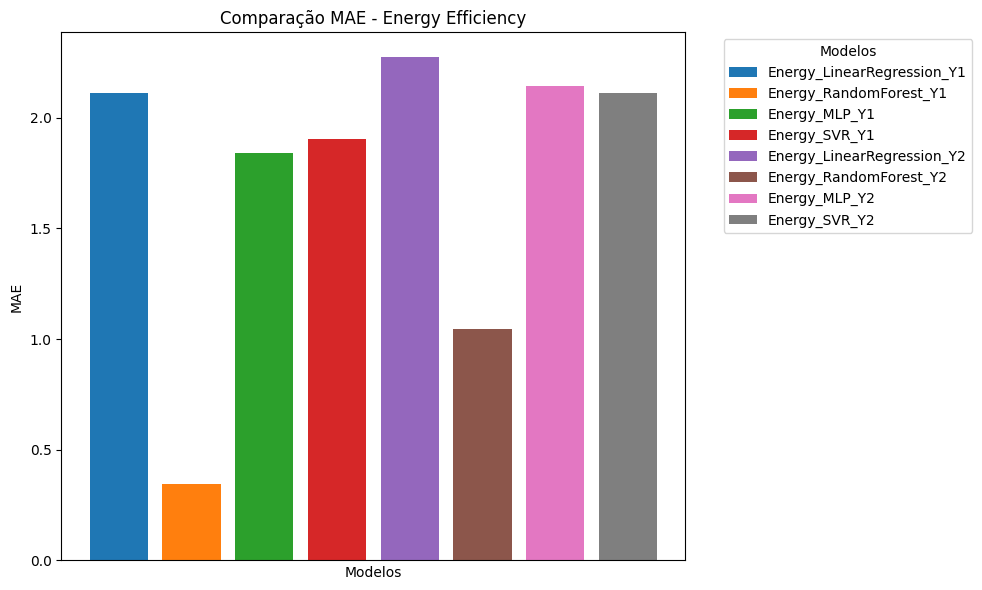
\includegraphics[width=0.45\textwidth]{../graficos/comparacao_mae_energy.png}
    \caption{Boxplot do MAE médio entre algoritmos de regressão para Energy Efficiency.}
    \label{fig:energy_mae}
\end{figure}

\begin{figure}[H]
    \centering
    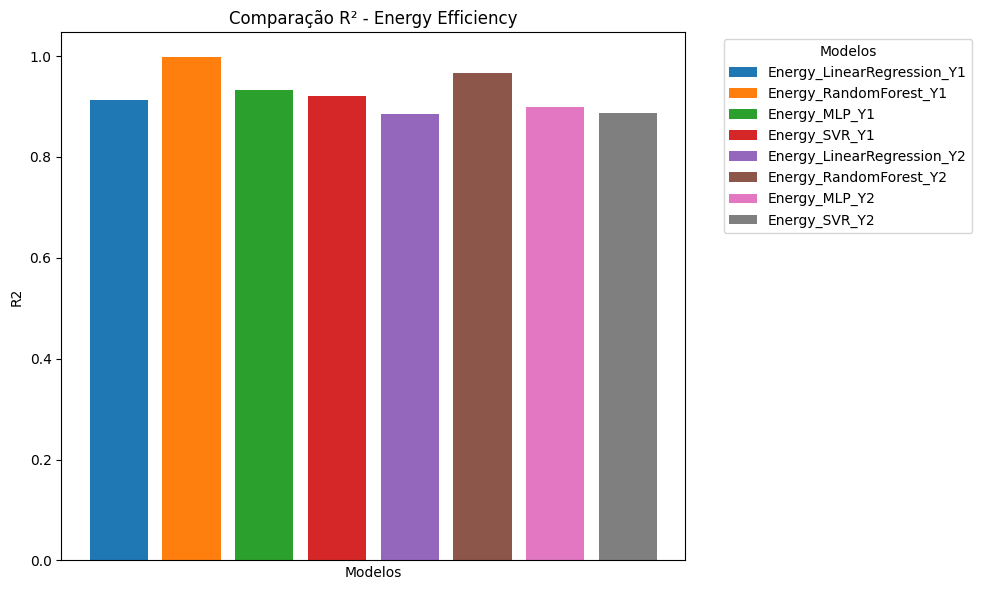
\includegraphics[width=0.45\textwidth]{../graficos/comparacao_r2_energy.png}
    \caption{Boxplot do $R^2$ médio entre algoritmos de regressão para Energy Efficiency.}
    \label{fig:energy_r2}
\end{figure}

No caso do California Housing, o comportamento dos algoritmos também varia, reforçando a importância de uma análise contextualizada. As Figuras~\ref{fig:california_rmse}, \ref{fig:california_mae} e \ref{fig:california_r2} apresentam, respectivamente, os boxplots de RMSE, MAE e $R^2$ para cada modelo. Essa visualização permite comparar rapidamente o desempenho dos algoritmos e identificar quais apresentam menor erro ou maior explicabilidade para essa base específica.

\begin{figure}[H]
    \centering
    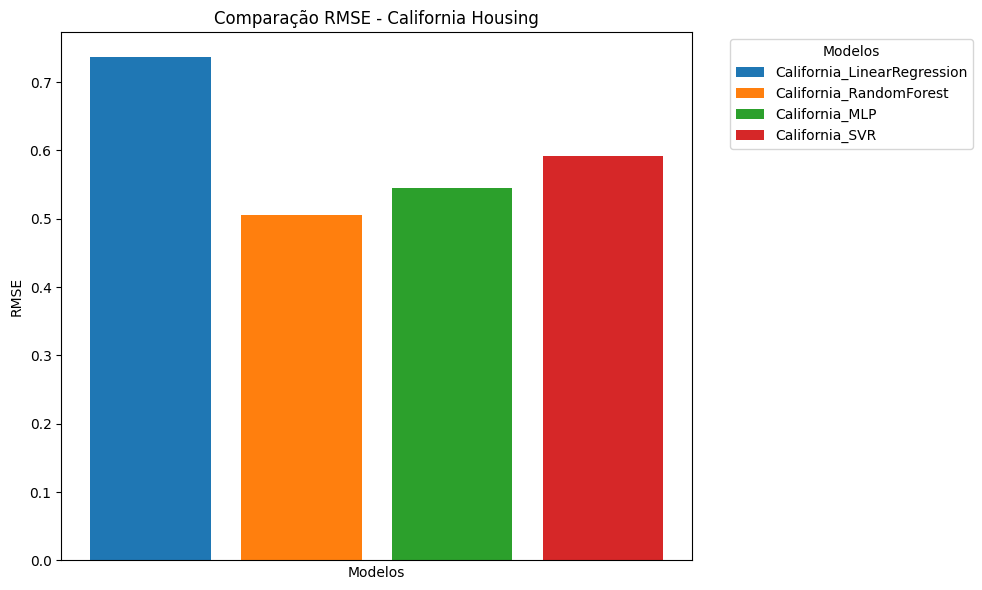
\includegraphics[width=0.45\textwidth]{../graficos/comparacao_rmse_california.png}
    \caption{Boxplot do RMSE médio entre algoritmos de regressão para California Housing.}
    \label{fig:california_rmse}
\end{figure}

\begin{figure}[H]
    \centering
    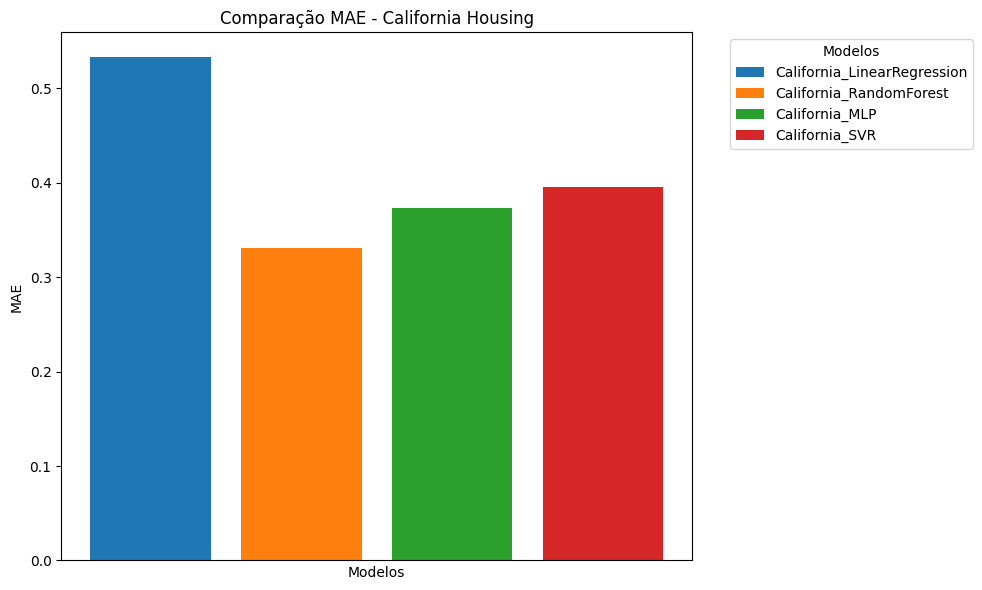
\includegraphics[width=0.45\textwidth]{../graficos/comparacao_mae_california.png}
    \caption{Boxplot do MAE médio entre algoritmos de regressão para California Housing.}
    \label{fig:california_mae}
\end{figure}

\begin{figure}[H]
    \centering
    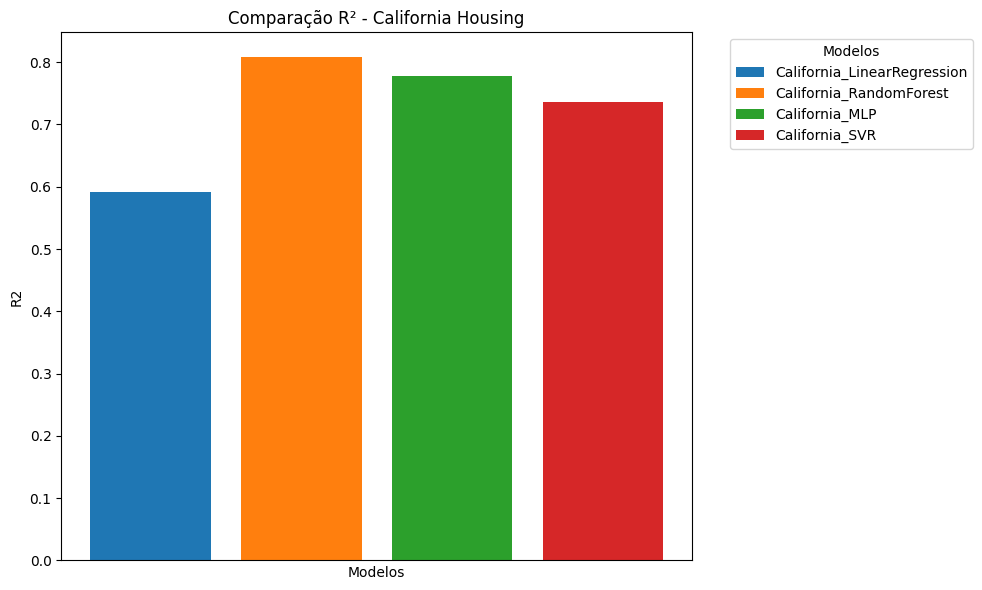
\includegraphics[width=0.45\textwidth]{../graficos/comparacao_r2_california.png}
    \caption{Boxplot do $R^2$ médio entre algoritmos de regressão para California Housing.}
    \label{fig:california_r2}
\end{figure}

\subsection{Análise dos Resultados de Classificação}

Na base Wine Quality sem balanceamento, nota-se diferenças relevantes entre os métodos, especialmente em métricas que consideram o equilíbrio entre as classes, como F1-score e Kappa. As Figuras~\ref{fig:wine_sem_bal_acuracia}, \ref{fig:wine_sem_bal_f1} e \ref{fig:wine_sem_bal_kappa} apresentam, respectivamente, os boxplots de acurácia, F1-score e Kappa para cada algoritmo. Isso permite comparar não só o desempenho geral, mas também a robustez dos modelos frente ao desbalanceamento das classes.

\begin{figure}[H]
    \centering
    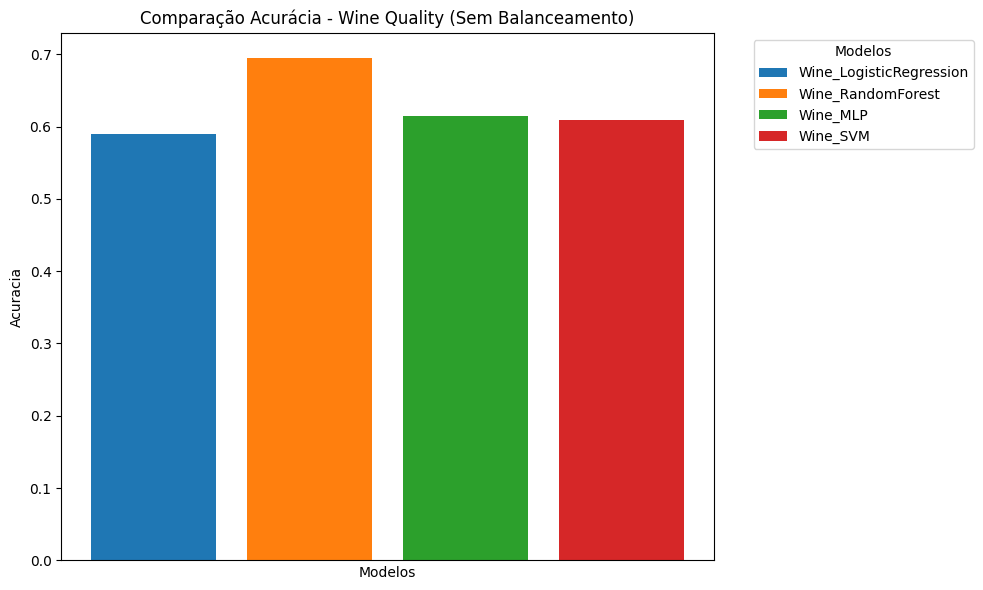
\includegraphics[width=0.45\textwidth]{../graficos/comparacao_acuracia_wine_sem_balanceamento.png}
    \caption{Boxplot da acurácia média entre algoritmos de classificação para Wine Quality (sem balanceamento).}
    \label{fig:wine_sem_bal_acuracia}
\end{figure}

\begin{figure}[H]
    \centering
    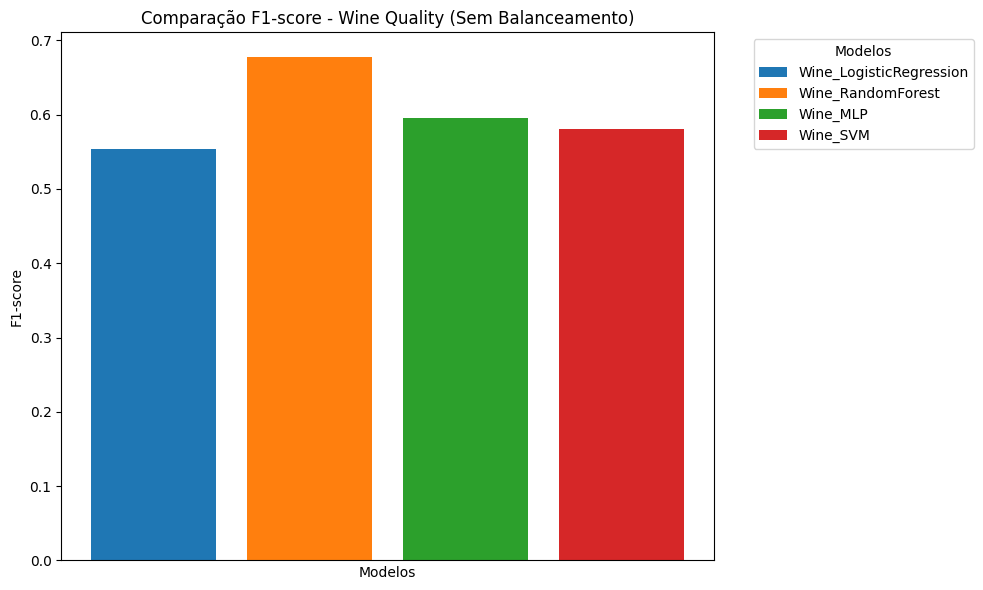
\includegraphics[width=0.45\textwidth]{../graficos/comparacao_f1_wine_sem_balanceamento.png}
    \caption{Boxplot do F1-score médio entre algoritmos de classificação para Wine Quality (sem balanceamento).}
    \label{fig:wine_sem_bal_f1}
\end{figure}

\begin{figure}[H]
    \centering
    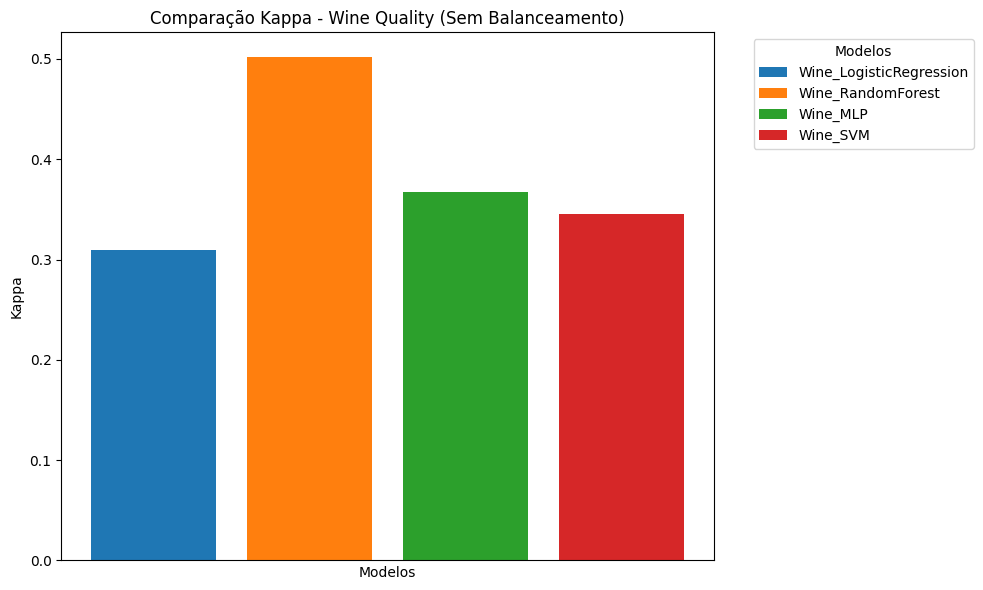
\includegraphics[width=0.45\textwidth]{../graficos/comparacao_kappa_wine_sem_balanceamento.png}
    \caption{Boxplot do Kappa médio entre algoritmos de classificação para Wine Quality (sem balanceamento).}
    \label{fig:wine_sem_bal_kappa}
\end{figure}

Mesmo em bases mais equilibradas, como a Iris, há variação entre os algoritmos, o que reforça a necessidade de avaliar múltiplas métricas. As Figuras~\ref{fig:iris_sem_bal_acuracia}, \ref{fig:iris_sem_bal_f1} e \ref{fig:iris_sem_bal_kappa} mostram, respectivamente, os boxplots de acurácia, F1-score e Kappa para os modelos testados na base Iris sem balanceamento, evidenciando diferenças de desempenho e estabilidade entre eles.

\begin{figure}[H]
    \centering
    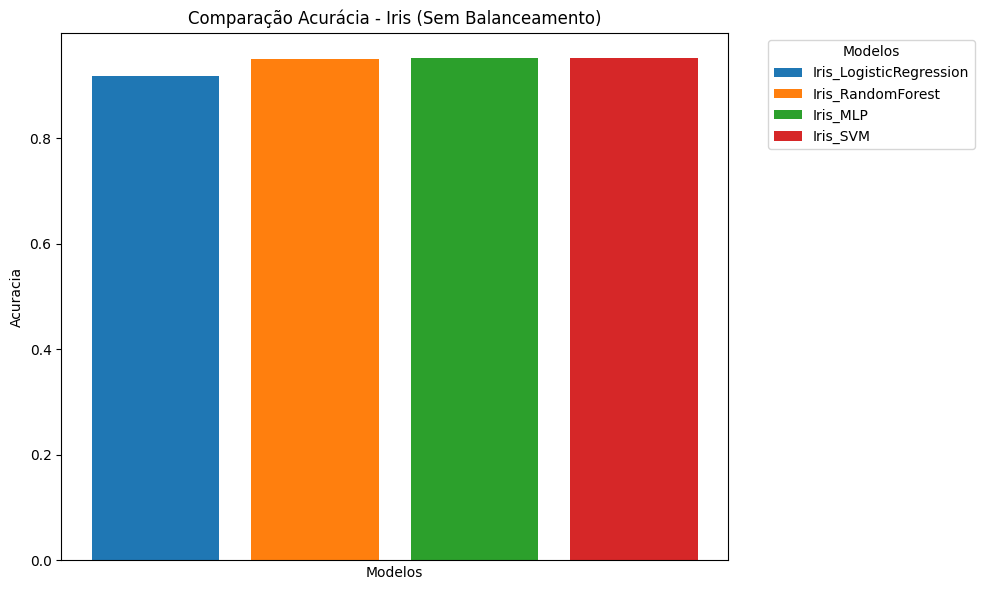
\includegraphics[width=0.45\textwidth]{../graficos/comparacao_acuracia_iris_sem_balanceamento.png}
    \caption{Boxplot da acurácia média entre algoritmos de classificação para Iris (sem balanceamento).}
    \label{fig:iris_sem_bal_acuracia}
\end{figure}

\begin{figure}[H]
    \centering
    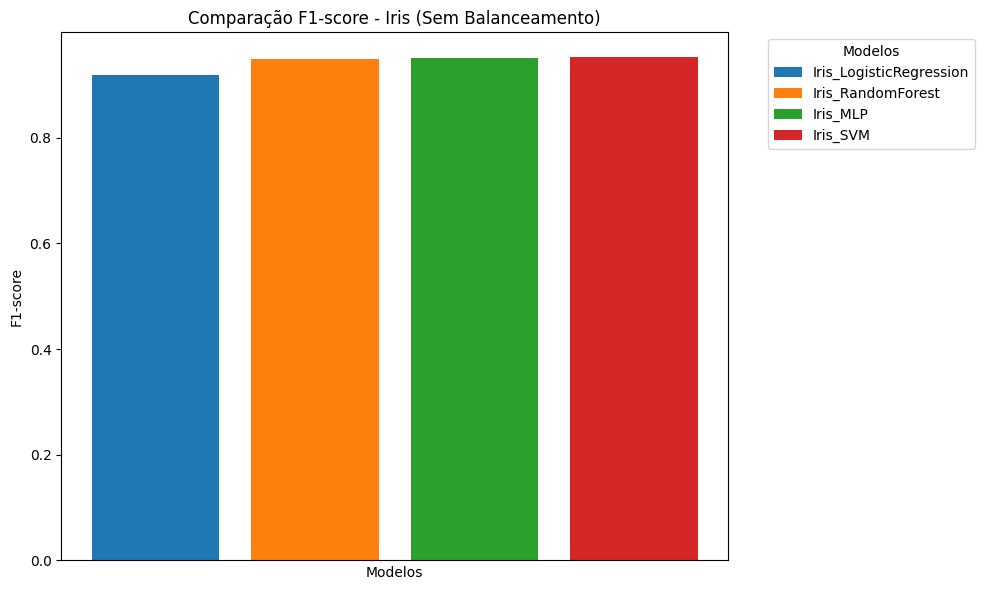
\includegraphics[width=0.45\textwidth]{../graficos/comparacao_f1_iris_sem_balanceamento.png}
    \caption{Boxplot do F1-score médio entre algoritmos de classificação para Iris (sem balanceamento).}
    \label{fig:iris_sem_bal_f1}
\end{figure}

\begin{figure}[H]
    \centering
    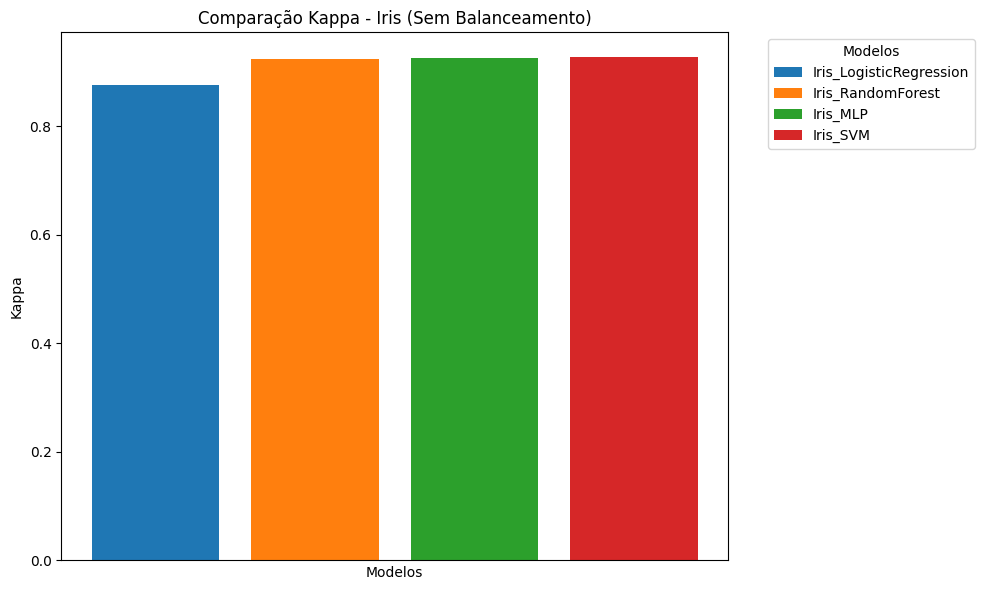
\includegraphics[width=0.45\textwidth]{../graficos/comparacao_kappa_iris_sem_balanceamento.png}
    \caption{Boxplot do Kappa médio entre algoritmos de classificação para Iris (sem balanceamento).}
    \label{fig:iris_sem_bal_kappa}
\end{figure}

Ao aplicar o balanceamento nas bases, nota-se mudanças no desempenho dos algoritmos, principalmente em métricas como F1-score e Kappa, tornando a comparação mais justa. As Figuras~\ref{fig:wine_com_bal_acuracia}, \ref{fig:wine_com_bal_f1} e \ref{fig:wine_com_bal_kappa} apresentam os boxplots de acurácia, F1-score e Kappa para a base Wine Quality com balanceamento, enquanto as Figuras~\ref{fig:iris_com_bal_acuracia}, \ref{fig:iris_com_bal_f1} e \ref{fig:iris_com_bal_kappa} mostram os mesmos indicadores para a base Iris balanceada. Essas visualizações evidenciam os ganhos proporcionados pelo balanceamento, especialmente na redução da variabilidade e no aumento da robustez dos modelos.

\begin{figure}[H]
    \centering
    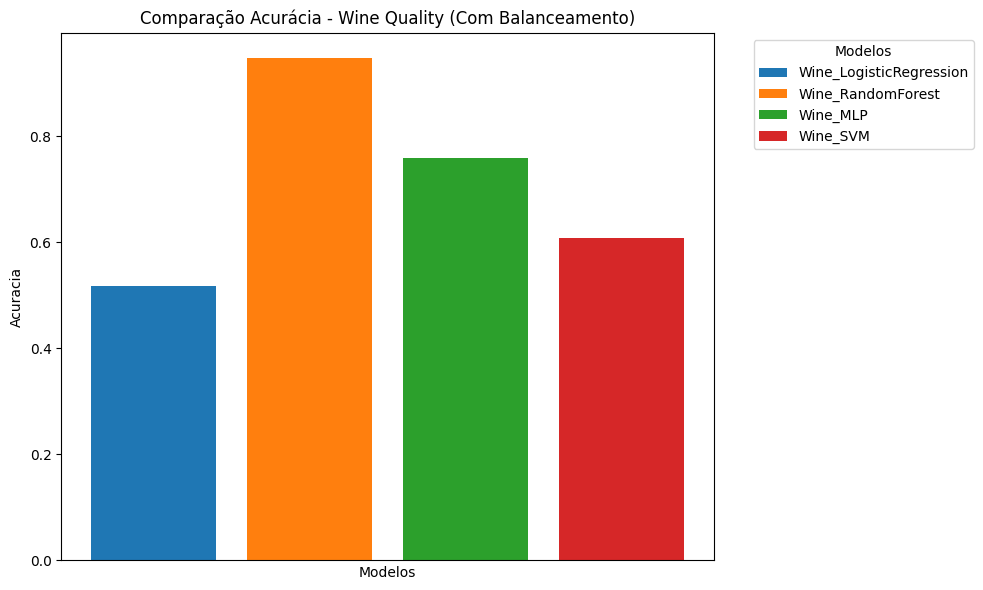
\includegraphics[width=0.45\textwidth]{../graficos/comparacao_acuracia_wine_com_balanceamento.png}
    \caption{Boxplot da acurácia média entre algoritmos de classificação para Wine Quality (com balanceamento).}
    \label{fig:wine_com_bal_acuracia}
\end{figure}

\begin{figure}[H]
    \centering
    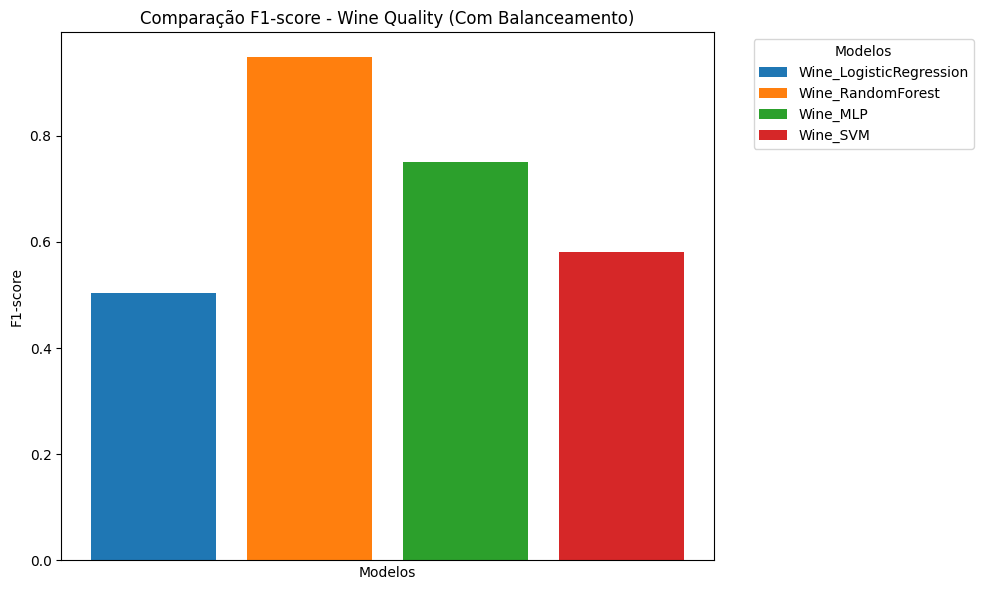
\includegraphics[width=0.45\textwidth]{../graficos/comparacao_f1_wine_com_balanceamento.png}
    \caption{Boxplot do F1-score médio entre algoritmos de classificação para Wine Quality (com balanceamento).}
    \label{fig:wine_com_bal_f1}
\end{figure}

\begin{figure}[H]
    \centering
    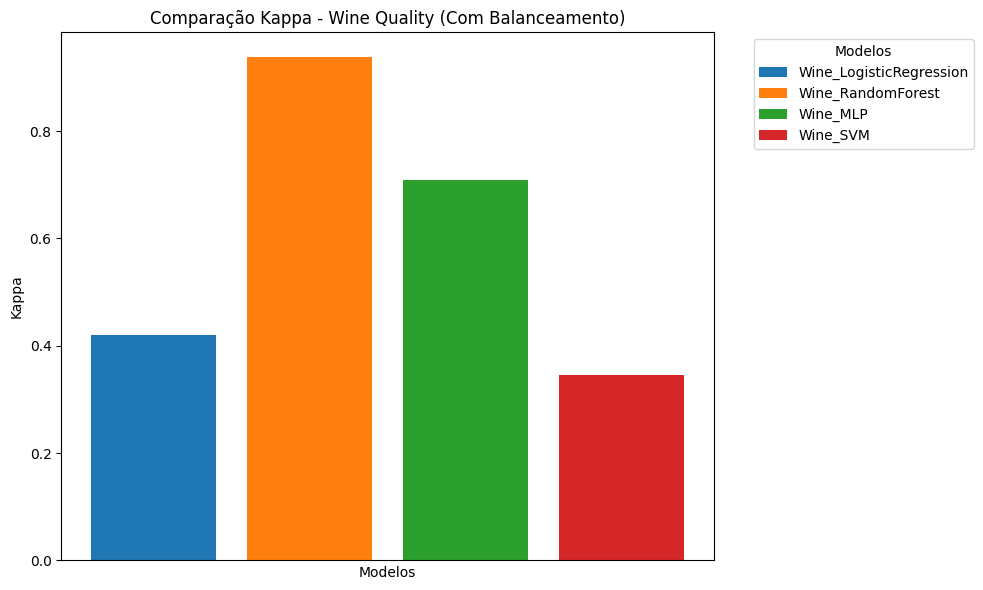
\includegraphics[width=0.45\textwidth]{../graficos/comparacao_kappa_wine_com_balanceamento.png}
    \caption{Boxplot do Kappa médio entre algoritmos de classificação para Wine Quality (com balanceamento).}
    \label{fig:wine_com_bal_kappa}
\end{figure}

\begin{figure}[H]
    \centering
    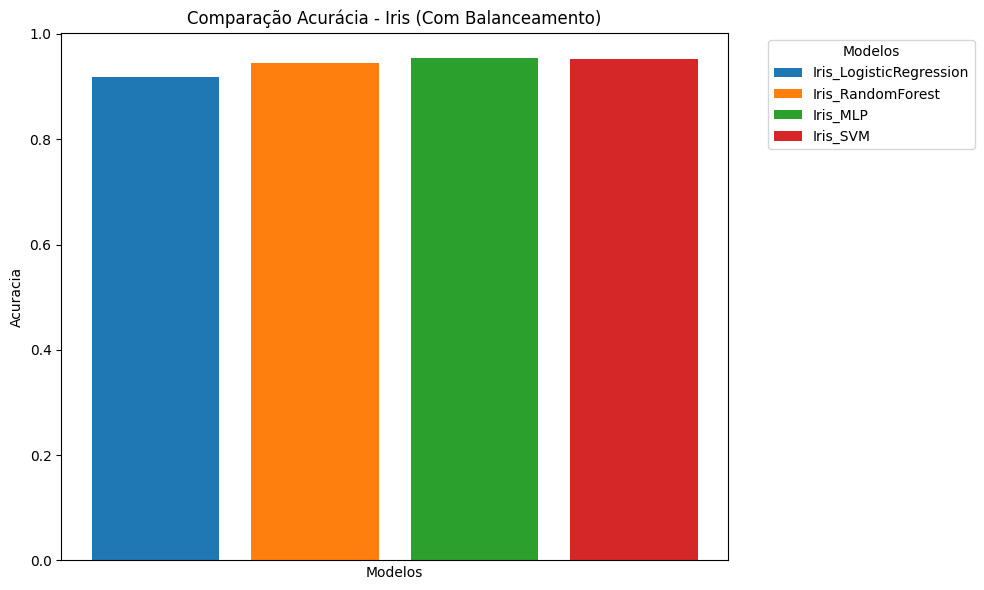
\includegraphics[width=0.45\textwidth]{../graficos/comparacao_acuracia_iris_com_balanceamento.png}
    \caption{Boxplot da acurácia média entre algoritmos de classificação para Iris (com balanceamento).}
    \label{fig:iris_com_bal_acuracia}
\end{figure}

\begin{figure}[H]
    \centering
    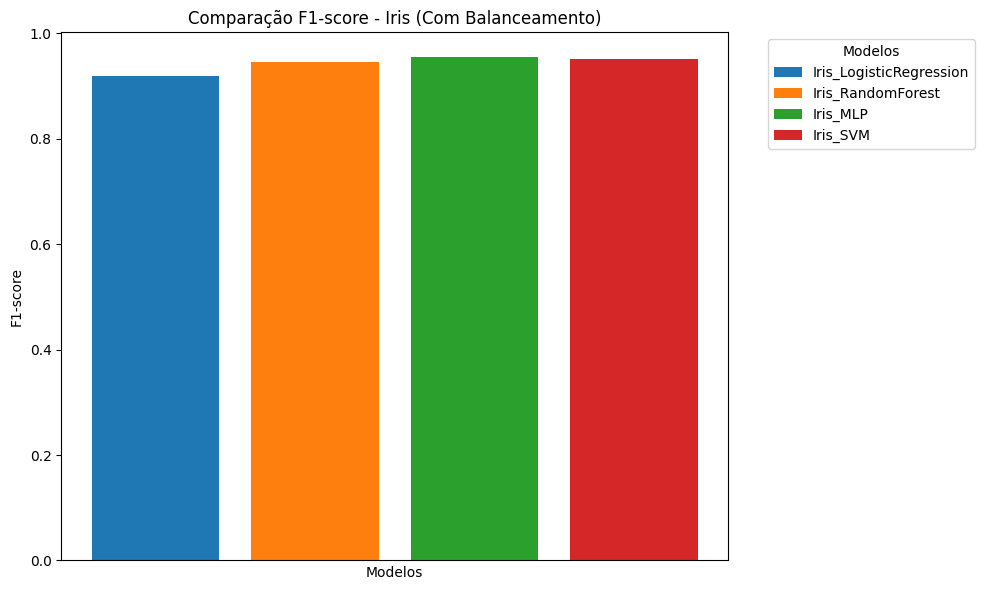
\includegraphics[width=0.45\textwidth]{../graficos/comparacao_f1_iris_com_balanceamento.png}
    \caption{Boxplot do F1-score médio entre algoritmos de classificação para Iris (com balanceamento).}
    \label{fig:iris_com_bal_f1}
\end{figure}

\begin{figure}[H]
    \centering
    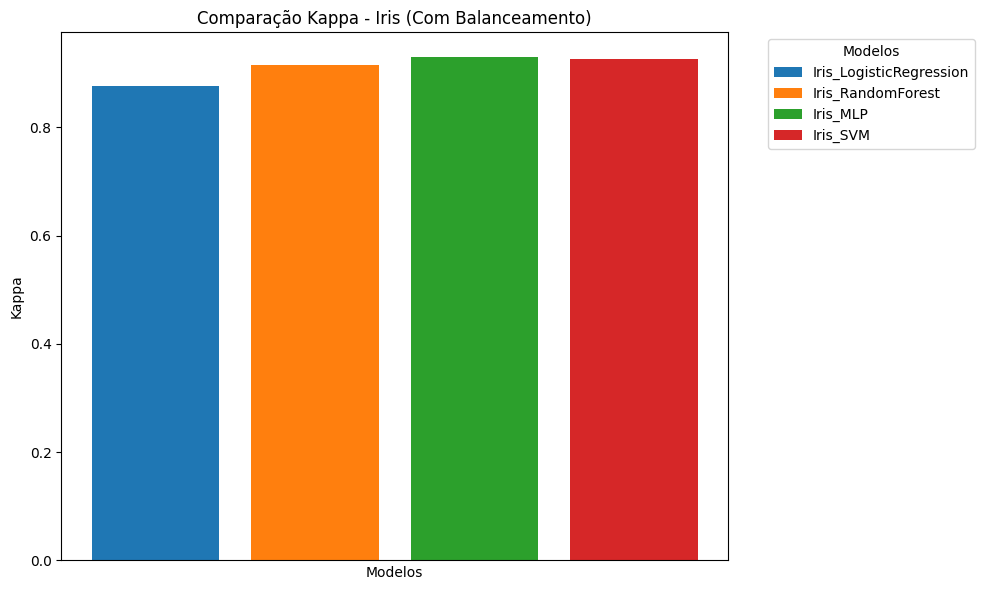
\includegraphics[width=0.45\textwidth]{../graficos/comparacao_kappa_iris_com_balanceamento.png}
    \caption{Boxplot do Kappa médio entre algoritmos de classificação para Iris (com balanceamento).}
    \label{fig:iris_com_bal_kappa}
\end{figure}


\subsection*{Síntese dos Resultados}

A análise dos resultados permite identificar, de forma clara e objetiva, quais algoritmos se destacaram positiva ou negativamente em cada cenário avaliado:

\begin{itemize}
    \item \textbf{Energy Efficiency (Regressão):} O Random Forest foi o modelo mais eficiente para ambos os alvos (Y1 e Y2), apresentando os menores valores de RMSE e MAE, além do maior $R^2$, o que indica excelente ajuste e baixa margem de erro. O Linear Regression, por sua vez, obteve os maiores erros e menor poder explicativo, especialmente para Y2.
    \item \textbf{California Housing (Regressão):} O Random Forest novamente se destacou, alcançando o menor RMSE, menor MAE e maior $R^2$. O Linear Regression apresentou o pior desempenho, com os maiores valores de erro e menor capacidade explicativa.
    \item \textbf{Wine Quality (Classificação, sem balanceamento):} O Random Forest foi o algoritmo mais eficaz, obtendo os maiores valores de acurácia, F1-score e Kappa. O Logistic Regression apresentou o pior desempenho geral, com os menores valores nessas métricas.
    \item \textbf{Wine Quality (Classificação, com balanceamento):} O Random Forest manteve o melhor desempenho, superando os demais algoritmos em acurácia, F1-score e Kappa. O Logistic Regression continuou com os piores resultados, especialmente em acurácia e F1-score.
    \item \textbf{Iris (Classificação, sem balanceamento):} Todos os métodos apresentaram desempenho elevado, mas MLP e SVM obtiveram os melhores resultados, com acurácia e F1-score de 0.9522 e Kappa acima de 0.925. O Logistic Regression, embora com desempenho um pouco inferior, ainda apresentou resultados satisfatórios.
    \item \textbf{Iris (Classificação, com balanceamento):} O MLP foi o destaque, com acurácia, F1-score e Kappa ligeiramente superiores aos demais. O Logistic Regression novamente apresentou os menores valores, mas a diferença entre os métodos foi pequena devido ao bom balanceamento e à simplicidade do dataset.
\end{itemize}

De maneira geral, o Random Forest mostrou-se o algoritmo mais robusto e eficiente para tarefas de regressão e classificação em cenários complexos ou desbalanceados. Já o MLP e o SVM se destacaram em bases bem comportadas, como a Iris. O Logistic Regression, apesar de sua simplicidade e interpretabilidade, apresentou desempenho inferior nos cenários mais desafiadores, mas ainda assim foi competitivo em bases balanceadas e de menor complexidade.